\Problem{Represetations of Vectors}{\VecRepsI}{
Discuss \textbf{vectors} with your group.
}
\ProblemSub{\VecRepsII}{
Write down a list of things about vectors on your shared whiteboard. You can write:
\begin{itemize}
	\item words or sentences
	\item numbers or symbols
	\item pictures or diagrams
\end{itemize}
Write large!
}
\Solution{\VecRepsSol}{

The following list only contains my thoughts about vectors. It should not be assumed to be definitive. There are many other things about vectors that could have been included.
\begin{itemize}
	\item A vector has direction and magnitude.
	\item A vector is often represented with an arrow; the length is its magnitude, and the orientation of the arrow (its angle) indicates direction.
	\begin{center}
		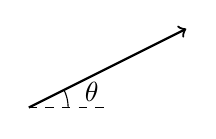
\begin{tikzpicture}
			\draw[thick,->] (0,0) -- (2,1);
			\draw[dashed] (0,0) -- (1,0);
			\draw (0.5,0) arc (0:27:0.5);
			\node at (0.8,0.2) {$\theta$};
		\end{tikzpicture}
	\end{center}
	\item Vectors add ``tip-to-tail.''
	\begin{center}
		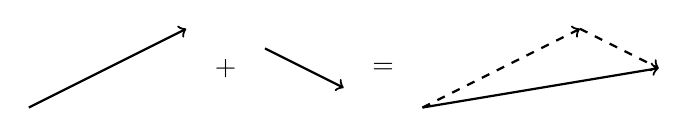
\begin{tikzpicture}
			\draw[thick,->] (0,0) -- (2,1);
			\node at (2.5,0.5) {$+$};
			\draw[thick,->,shift={(3,0)}] (0,0.75) -- (1,0.25);
			\node at (4.5,0.5) {$=$};
			\draw[thick,->,shift={(5,0)}] (0,0) -- (3,0.5);
			\draw[thick,dashed,->,shift={(5,0)}] (0,0) -- (2,1);
			\draw[thick,dashed,->,shift={(7,0.25)}] (0,0.75) -- (1,0.25);
		\end{tikzpicture}
	\end{center}
	\item Multiplying a vector by a scalar changes its length.
	\begin{center}
		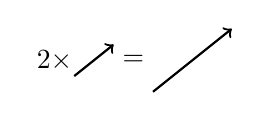
\begin{tikzpicture}
			\node at (0,0) {$2\times$};
			\draw[thick,->] (0.25,-0.2) -- (0.75,0.2);
			\node at (1,0) {$=$};
			\draw[thick,->] (1.25,-0.4) -- (2.25,0.4);
		\end{tikzpicture}
	\end{center}
	\item Multiplying a vector by $-1$ reverses its direction.
	\begin{center}
		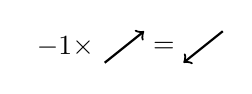
\begin{tikzpicture}
			\node at (-0.25,0) {$-1\times$};
			\draw[thick,->] (0.25,-0.2) -- (0.75,0.2);
			\node at (1,0) {$=$};
			\draw[thick,->] (1.75,0.2) -- (1.25,-0.2);
		\end{tikzpicture}
	\end{center}
	\item Vectors can be broken into components.
	\begin{center}
		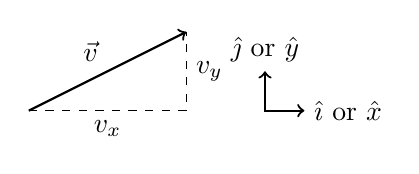
\begin{tikzpicture}
			\draw[thick,->] (0,0) -- (2,1);
			\node[anchor=south east] at (1,0.5) {$\vec{v}$};
			\draw[dashed] (0,0) -- (2,0) -- (2,1);
			\node[anchor=north] at (1,0) {$v_{x}$};
			\node[anchor=west] at (2,0.5) {$v_{y}$};
			\draw[<->,thick] (3,0.5) -- (3,0) -- (3.5,0);
			\node[anchor=south] at (3,0.5) {$\hat{\jmath}$ or $\hat{y}$};
			\node[anchor=west] at (3.5,0) {$\hat{\imath}$ or $\hat{x}$};
		\end{tikzpicture}
	\end{center}
	Parenthetical or angle-bracket notation was probably used in your math classes:
	\[
	\vec{v} = (v_{x},v_{y}) = \langle v_{x},v_{y}\rangle.
	\]
	It is okay, but parentheses and angle brackets can mean a lot of things, so it may not always be clear. \\
	We recommend unit vector notation, as it is much clearer:
	\[
	\vec{v} = v_{x}\hat{\imath} + v_{y}\hat{\jmath} = v_{x}\hat{x} + v_{y}\hat{y}.
	\]
	Using $\hat{x}$, $\hat{y}$, $\hat{z}$ instead of $\hat{\imath}$, $\hat{\jmath}$, $\hat{k}$ helps to more clearly associate the Cartesian unit vectors with the coordinate axes. \\
	\textbf{Warning!} Cosine is not always $x$! It depends on where the angle is.
	\begin{center}
		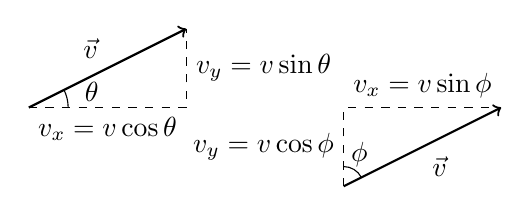
\begin{tikzpicture}
			\begin{scope}[shift={(-2,0.5)}]
				\draw[thick,->] (0,0) -- (2,1);
				\node[anchor=south east] at (1,0.5) {$\vec{v}$};
				\draw[dashed] (0,0) -- (2,0) -- (2,1);
				\draw (0.5,0) arc (0:27:0.5);
				\node at (0.8,0.2) {$\theta$};
				\node[anchor=north] at (1,0) {$v_{x}=v\cos\theta$};
				\node[anchor=west] at (2,0.5) {$v_{y}=v\sin\theta$};
			\end{scope}
			\begin{scope}[shift={(2,-0.5)}]
				\draw[thick,->] (0,0) -- (2,1);
				\node[anchor=north west] at (1,0.5) {$\vec{v}$};
				\draw[dashed] (0,0) -- (0,1) -- (2,1);
				\draw (0,0.25) arc (90:27:0.25);
				\node at (0.2,0.4) {$\phi$};
				\node[anchor=south] at (1,1) {$v_{x}=v\sin\phi$};
				\node[anchor=east] at (0,0.5) {$v_{y}=v\cos\phi$};
			\end{scope}
		\end{tikzpicture}
	\end{center}
	\item Vectors add ``componentwise.''
	\begin{center}
		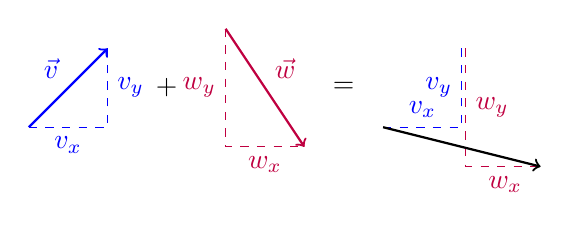
\begin{tikzpicture}
			\begin{scope}[blue,shift={(0,0)}]
				\draw[thick,->] (0,0) -- (1,1);
				\node[anchor=south east] at (0.5,0.5) {$\vec{v}$};
				\draw[dashed] (0,0) -- (1,0) -- (1,1);
				\node[anchor=north] at (0.5,0) {$v_{x}$};
				\node[anchor=west] at (1,0.5) {$v_{y}$};
			\end{scope}
			\node at (1.75,0.5) {$+$};
			\begin{scope}[purple,shift={(2.5,0.25)}]
				\draw[thick,->] (0,1) -- (1,-0.5);
				\node[anchor=south west] at (0.5,0.25) {$\vec{w}$};
				\draw[dashed] (0,1) -- (0,-0.5) -- (1,-0.5);
				\node[anchor=north] at (0.5,-0.5) {$w_{x}$};
				\node[anchor=east] at (0,0.25) {$w_{y}$};
			\end{scope}
			\node at (4,0.5) {$=$};
			\begin{scope}[blue,shift={(4.5,0)}]
				%\draw[thick,->] (0,0) -- (1,1);
				%\node[anchor=south east] at (0.5,0.5) {$\vec{v}$};
				\draw[dashed] (0,0) -- (1,0) -- (1,1);
				\node[anchor=south] at (0.5,0) {$v_{x}$};
				\node[anchor=east] at (1,0.5) {$v_{y}$};
			\end{scope}
			\begin{scope}[purple,shift={(5.55,0)}]
				%\draw[thick,->] (0,1) -- (1,-0.5);
				%\node[anchor=south west] at (0.5,0.25) {$\vec{w}$};
				\draw[dashed] (0,1) -- (0,-0.5) -- (0.95,-0.5);
				\node[anchor=north] at (0.5,-0.5) {$w_{x}$};
				\node[anchor=west] at (0,0.25) {$w_{y}$};
			\end{scope}
			\draw[thick,->] (4.5,0) -- (6.5,-0.5);
		\end{tikzpicture}
	\end{center}
	\[
	{\color{blue}\vec{v}} + {\color{purple}\vec{w}} = {\color{blue}v_{x}\hat{x}+v_{y}\hat{y}} + {\color{purple}w_{x}\hat{x}+w_{y}\hat{y}} = ({\color{blue}v_{x}}+{\color{purple}w_{x}})\hat{x} + ({\color{blue}v_{y}}+{\color{purple}w_{y}})\hat{y}
	\]
\end{itemize}
}